% Options for packages loaded elsewhere
\PassOptionsToPackage{unicode}{hyperref}
\PassOptionsToPackage{hyphens}{url}
%
\documentclass[
  letterpaper,
]{book}

\usepackage{amsmath,amssymb}
\usepackage{iftex}
\ifPDFTeX
  \usepackage[T1]{fontenc}
  \usepackage[utf8]{inputenc}
  \usepackage{textcomp} % provide euro and other symbols
\else % if luatex or xetex
  \usepackage{unicode-math}
  \defaultfontfeatures{Scale=MatchLowercase}
  \defaultfontfeatures[\rmfamily]{Ligatures=TeX,Scale=1}
\fi
\usepackage{lmodern}
\ifPDFTeX\else  
    % xetex/luatex font selection
\fi
% Use upquote if available, for straight quotes in verbatim environments
\IfFileExists{upquote.sty}{\usepackage{upquote}}{}
\IfFileExists{microtype.sty}{% use microtype if available
  \usepackage[]{microtype}
  \UseMicrotypeSet[protrusion]{basicmath} % disable protrusion for tt fonts
}{}
\makeatletter
\@ifundefined{KOMAClassName}{% if non-KOMA class
  \IfFileExists{parskip.sty}{%
    \usepackage{parskip}
  }{% else
    \setlength{\parindent}{0pt}
    \setlength{\parskip}{6pt plus 2pt minus 1pt}}
}{% if KOMA class
  \KOMAoptions{parskip=half}}
\makeatother
\usepackage{xcolor}
\setlength{\emergencystretch}{3em} % prevent overfull lines
\setcounter{secnumdepth}{5}
% Make \paragraph and \subparagraph free-standing
\ifx\paragraph\undefined\else
  \let\oldparagraph\paragraph
  \renewcommand{\paragraph}[1]{\oldparagraph{#1}\mbox{}}
\fi
\ifx\subparagraph\undefined\else
  \let\oldsubparagraph\subparagraph
  \renewcommand{\subparagraph}[1]{\oldsubparagraph{#1}\mbox{}}
\fi


\providecommand{\tightlist}{%
  \setlength{\itemsep}{0pt}\setlength{\parskip}{0pt}}\usepackage{longtable,booktabs,array}
\usepackage{calc} % for calculating minipage widths
% Correct order of tables after \paragraph or \subparagraph
\usepackage{etoolbox}
\makeatletter
\patchcmd\longtable{\par}{\if@noskipsec\mbox{}\fi\par}{}{}
\makeatother
% Allow footnotes in longtable head/foot
\IfFileExists{footnotehyper.sty}{\usepackage{footnotehyper}}{\usepackage{footnote}}
\makesavenoteenv{longtable}
\usepackage{graphicx}
\makeatletter
\def\maxwidth{\ifdim\Gin@nat@width>\linewidth\linewidth\else\Gin@nat@width\fi}
\def\maxheight{\ifdim\Gin@nat@height>\textheight\textheight\else\Gin@nat@height\fi}
\makeatother
% Scale images if necessary, so that they will not overflow the page
% margins by default, and it is still possible to overwrite the defaults
% using explicit options in \includegraphics[width, height, ...]{}
\setkeys{Gin}{width=\maxwidth,height=\maxheight,keepaspectratio}
% Set default figure placement to htbp
\makeatletter
\def\fps@figure{htbp}
\makeatother

\usepackage{makeidx}
\makeindex
\makeatletter
\@ifpackageloaded{bookmark}{}{\usepackage{bookmark}}
\makeatother
\makeatletter
\@ifpackageloaded{caption}{}{\usepackage{caption}}
\AtBeginDocument{%
\ifdefined\contentsname
  \renewcommand*\contentsname{Table of contents}
\else
  \newcommand\contentsname{Table of contents}
\fi
\ifdefined\listfigurename
  \renewcommand*\listfigurename{List of Figures}
\else
  \newcommand\listfigurename{List of Figures}
\fi
\ifdefined\listtablename
  \renewcommand*\listtablename{List of Tables}
\else
  \newcommand\listtablename{List of Tables}
\fi
\ifdefined\figurename
  \renewcommand*\figurename{Figure}
\else
  \newcommand\figurename{Figure}
\fi
\ifdefined\tablename
  \renewcommand*\tablename{Table}
\else
  \newcommand\tablename{Table}
\fi
}
\@ifpackageloaded{float}{}{\usepackage{float}}
\floatstyle{ruled}
\@ifundefined{c@chapter}{\newfloat{codelisting}{h}{lop}}{\newfloat{codelisting}{h}{lop}[chapter]}
\floatname{codelisting}{Listing}
\newcommand*\listoflistings{\listof{codelisting}{List of Listings}}
\makeatother
\makeatletter
\makeatother
\makeatletter
\@ifpackageloaded{caption}{}{\usepackage{caption}}
\@ifpackageloaded{subcaption}{}{\usepackage{subcaption}}
\makeatother
\ifLuaTeX
  \usepackage{selnolig}  % disable illegal ligatures
\fi
\usepackage{bookmark}

\IfFileExists{xurl.sty}{\usepackage{xurl}}{} % add URL line breaks if available
\urlstyle{same} % disable monospaced font for URLs
\hypersetup{
  pdftitle={International Macroeconomics: Lecture Notes},
  pdfauthor={Udayan Roy},
  hidelinks,
  pdfcreator={LaTeX via pandoc}}

\title{International Macroeconomics: Lecture Notes}
\author{Udayan Roy}
\date{2024-07-14}

\begin{document}
\frontmatter
\maketitle

\renewcommand*\contentsname{Table of contents}
{
\setcounter{tocdepth}{2}
\tableofcontents
}
\mainmatter
\bookmarksetup{startatroot}

\chapter*{Preface}\label{preface}
\addcontentsline{toc}{chapter}{Preface}

\markboth{Preface}{Preface}

These lecture notes are for a very short course---roughly twelve
75-minute lectures---on international macroeconomics that I have taught
to junior and senior undergraduates. Although no prior knowledge of
economics is assumed, students typically come to the course after
completing courses on introductory microeconomics and macroeconomics.

This course is the second half of a one-semester course on international
economics, with the first half on international trade. The course's
textbook is \emph{International Economics: Theory and Policy}, Twelfth
Edition, by Paul R. Krugman\index{Krugman, Paul R.}, Maurice
Obstfeld\index{Obstfeld, Maurice}, and Marc J.
Melitz\index{Melitz, Marc}, Pearson, 2022, ISBN 9780135766859. My goal
here is simply to present a concise version of chapters 13 through 18 of
that book.

I had to grapple with some tough trade-offs because of the severe time
constraint. The core of the course is the theoretical framework
originally proposed by Robert A. Mundell\index{Mundell, Robert A.} and
J. Marcus Fleming\index{Fleming, J. Marcus}. I assume perfect capital
mobility\index{perfect capital mobility} throughout and, thereby, avoid
all discussion of wealth effects and portfolio theory.\footnote{On these
  issues, see \emph{Open Economy Macroeconomics} by Asbj\{\o\}rn
  R\{\o\}dseth\index{R{\o}dseth, Asbj{\o}rn}, Cambridge University
  Press, Cambridge, UK, 2000, ISBN 0-521-78304-6 (hardback) and
  0-521-78874-9 (paperback). By perfect capital
  mobility\index{perfect capital mobility} I mean a world in which (a)
  people who buy assets care only about the expected returns of those
  assets, and (b) they all have the same expectations about future
  changes in exchange rates. See section XXX.} I also assume a ``small''
country and, thereby, avoid the complex interactions of two-country
models. The perfect capital mobility and small country assumptions keep
this course very similar to the undergraduate macroeconomics course that
most of my students would have also taken. This simplicity, I think,
allows students to focus on the special aspects of \emph{international}
macroeconomics without having to learn a new kind of macroeconomics.

However, the discussion of expectations here may surprise even students
who have taken intermediate macroeconomics courses. I have broken up the
discussion of short-run analysis into separate chapters on permanent and
temporary changes in exogenous variables. Expectations are assumed to be
anchored to the long-run equilibrium outcome. This assumption is at the
root of the need to distinguish between temporary and permanent changes
in, say, fiscal policy. A temporary change affects neither the long-run
equilibrium outcome nor people's expectations, which are, after all,
assumed to be tied to the long-run equilibrium outcome. On the other
hand, a permanent change in, say, government spending affects the
long-run equilibrium level of the future value of the exchange rate and,
consequently, people's expectations about the future value of the
exchange rate. This change in expectations has short-run ramifications
that are absent in the analysis of temporary changes in government
spending.

These notions are present in the book by Krugman, Obstfeld, and Melitz,
but are not developed in a way that is clear enough and leisurely enough
for most students to grasp.\footnote{On page 442 of their book, Krugman,
  Obstfeld, and Melitz address the issue as follows: ``A permanent
  policy shift affects not only the current value of the government's
  policy instrument (the money supply, government spending, or taxes)
  but also the \emph{long-run} exchange rate. This in turn affects
  expectations about future exchange rates. Because these changes in
  expectations have a major influence on the exchange rate prevailing in
  the short run, the effects of permanent policy shifts differ from
  those of temporary shifts.''} Other international macroeconomics
textbooks are no better in this respect, and usually a lot
worse.\footnote{Consider \emph{International Economics}, by Robert C.
  Feenstra and Alan M. Taylor, Worth Publishers, New York, NY, 2008,
  ISBN 0-7167-9283-4. On page 551 of their excellent textbook, the
  authors write, ``{[}W{]}e can form expectations of the future exchange
  rate using the long-run monetary approach \ldots{}'' This easy-to-miss
  mention of the idea that expectations are based on the long-run
  equilibrium outcome is not adequately developed, as far as I am
  concerned. And the consequent need to distinguish between temporary
  and permanent policy changes is not as clearly developed as I would
  like.}

The role of the long-run outcome in anchoring expectations is also my
reason to discuss the long run before the short run. It would be
essentially impossible to do short-run analysis without some notion of
how expectations are formed, and the formation of expectations would be
impossible to explain without a discussion of long-run equilibrium.

These lecture notes are a work in progress. Readers are encouraged to
suggest improvements or at the very least send in some angry comments.
My mailing address is Udayan Roy, College of Management, Long Island
University, Brookville, NY 11548, USA. My email address is
\href{mailto:udayan.roy@liu.edu}{\nolinkurl{udayan.roy@liu.edu}}.

\bookmarksetup{startatroot}

\chapter{Preliminaries}\label{sec-preliminaries}

\section{Economics}\label{sec-economics}

Economics\index{economics} is the study of how we---as individuals and
as societies---deal with the inescapable reality that ``we can't always
get what we want''. This fact of life, which economists call
\emph{scarcity}, makes it important for us to know how the many economic
variables that are important to us---such as the gross domestic product,
the unemployment rate, the consumer price index, etc.---can be made to
increase or decrease as needed. For example, scarcity makes it important
to understand whether our gross domestic product would increase or
decrease if we imposed tariffs on imported goods.

Economics consists of:

\begin{itemize}
\tightlist
\item
  \textbf{theories}, which are explanations---not necessarily
  proven---for the observed up and down movements of the economic
  variables that matter to us, and of
\item
  \textbf{statistical studies} that seek to test the reliability of
  economic theories.
\end{itemize}

\section{Macroeconomics}\label{sec-macro}

Macroeconomics\index{economics!macroeconomics} is the part of economics
that deals with economic variables that describe a country. When
describing the economy of the United States, an economist will probably
mention the gross domestic product, the unemployment rate, the inflation
rate, the trade deficit, etc., of the United States. These variables
that describe an entire country are at the heart of macroeconomics.
Macroeconomics consists of (a) theories that derive predictions about
the likely changes in such economic variables and (b) statistical
studies that scour history to check the predictive accuracy of the
theories.

\section{International Macroeconomics}\label{sec-intmac}

The macroeconomic behavior of a country that is economically isolated
from other countries---a \textbf{closed economy}, in the jargon of
economics---will not necessarily be the same as the macroeconomic
behavior of a highly globalized country---an \textbf{open economy}.
International macroeconomics is the part of macroeconomics that deals
with countries for which international economic links are important.
Such links may include international trade in goods and services,
cross-border migration of people, and cross-border borrowing and
lending.

\section{Why Study International Macroeconomics?}\label{sec-whyintmac}

The point of studying international macroeconomics is to be able to
\emph{evaluate alternative macroeconomic policies} and choose the one
that's best. If we have a reliable theory that explains the reasons why
a certain variable goes up or down, we might be able to figure out
policies that will move that variable in the desired direction. For
example, if we can figure out the reasons for the up and down movements
of a nation's trade deficit, we might be able to design economic
policies that drive the trade deficit in the desired direction, be it up
or down.

In discussing macroeconomic policy\index{policy} I will focus on
\textbf{fiscal policy} and \textbf{monetary policy}.

\subsection{What Is Fiscal Policy?}\label{sec-fiscal}

Fiscal policy\index{policy!fiscal policy} consists of all the methods of
controlling an economy by making changes to the government's budget. A
government's \textbf{budget}\index{budget, government's} is a
description of its spending and revenue-raising plans. So, for my
purposes, fiscal policy essentially consists of changes in total
\textbf{government spending}\index{government spending}, \(G\), and
\textbf{total tax revenue}\index{tax revenue}, \(T\).\footnote{First,
  note that I have begun to introduce symbols to denote economic
  variables. As you will see, the good part of the use of symbols is
  that it speeds up the discussion considerably. The bad part is that
  you will need to remember which symbol denotes which variable.}

Second, to be more precise, \(T\) represents total \emph{net} tax
revenue, which equals the tax revenues of the government less
\textbf{transfer payments} made by the government. Transfer payments are
gifts, such as cash grants to the poor.

Third, \(G\) represents government \emph{purchases} rather than
government spending. The latter includes the former plus transfer
payments, which, as I said in the previous paragraph, are gifts, not
payments made for purchases. \(G\) represents only what the government
spends for its purchases of goods and services.

\subsection{What Is Monetary Policy?}\label{sec-monetary}

Monetary policy\index{policy!monetary policy} consists of all the
methods of controlling an economy by making changes to the economic
variables that are directly controlled by the country's monetary
authorities, such as the Federal Reserve in the United States. For my
purposes, monetary policy consists of changes in a country's
\textbf{money supply}, \(M\). A central bank may print money and lend it
to financial institutions such as banks. If and when these financial
institutions in turn lend the money to people or to businesses, the
newly printed money begins to affect actual economic activity. This, of
course, is why the central bank printed the money in the first place.

\subsection{Monetary Unions}\label{sec-monetary-unions}

In the case of the 24 European countries that all use the same currency,
the euro, there is no monetary policy at all to conduct!\footnote{As of
  October 2023, the eurozone consists of 20 members who are European
  Union (EU) members and use the euro. They are Austria, Belgium,
  Croatia, Cyprus, Estonia, Finland, France, Germany, Greece, Ireland,
  Italy, Latvia, Lithuania, Luxembourg, Malta, the Netherlands,
  Portugal, Slovakia, Slovenia and Spain. The non-EU countries that use
  the euro are Andorra, Vatican City, and Monaco and San Marino.} These
countries have willingly given up their individual currencies and formed
a \textbf{monetary union}\index{European Monetary Union}. The monetary
policy of the entire eurozone is determined by the European Central
Bank\index{central banks!European Central Bank} in Frankfurt.\footnote{This
  lack of the ability to use monetary policy is also true of a handful
  of countries that have ``dollarized''\index{dollarization}. These are
  countries that have decided to use another country's currency as their
  own currency. For example, East Timor, Ecuador, El Salvador, and
  Panama use the U.S. dollar as their currency.}

It is important to understand the pros and cons of the formation of a
monetary union so that countries considering joining a monetary union
may make smart choices.

Just as multiple countries may choose to use a common currency, they may
also choose to adopt a common fiscal policy whereby a central budget
sets expenditure and revenue-raising rules for all members of the club.
For example, the USA may be thought of as a union of fifty states with a
common currency and a unified fiscal policy decided in Washington, D.C.
In fact, we will see that it may be difficult for a group of countries
to share a common currency and retain independent national fiscal
policies. During the economic crises that cascaded through several
eurozone countries---such as Ireland, Greece, and Spain---during
2009--2012, some commentators argued that the eurozone countries needed
to unify their budgets---and become something like a United States of
Europe---if they were to have a stable monetary union.

In any case, countries considering a monetary and/or fiscal union need
to be able to make their choices with their eyes wide open. It is,
therefore, necessary for international economics to have something
useful to say on the issue.

\bookmarksetup{startatroot}

\chapter{National Income Accounts, Prices, and
Inflation}\label{sec-niaccounts}

Recall from sections Section~\ref{sec-economics} --
Section~\ref{sec-intmac} that international macroeconomics consists of
explanations for the observed up-and-down movements of important
macroeconomic variables in a globalized (or, open) economy. This chapter
begins the task of defining some of those important macroeconomic
variables. This chapter also discusses certain accounting rules that
describe how certain important macroeconomic variables are related to
each other, simply by virtue of the way they are defined.

\section{National Income Accounts}\label{sec-nia}

The national income accounts of a country consist of data on variables
that tell us about the country's total production of goods and services,
and what those goods and services are being used for. An important
measure of the total production of goods and services is the gross
domestic product (GDP). If you look up a country's GDP data in a book or
on the Internet, you'll see that GDP data comes in two flavors, nominal
and real. Nominal GDP is discussed in the next section, and real GDP is
discussed in the section after that.

\section{\texorpdfstring{Nominal Gross Domestic Product \{\#sec-nGDP\}
\index{gross domestic product!nominal}}{Nominal Gross Domestic Product \{\#sec-nGDP\} }}\label{nominal-gross-domestic-product-sec-ngdp}

There are three equivalent ways of understanding nominal gross domestic
product: the value-added approach, the income approach, and the
expenditure approach.

\subsection{GDP: The Value-Added Approach}\label{sec-gdp-value-added}

The \textbf{value added}\index{value added} by a firm is the monetary
market value of the goods and services produced by the firm \emph{minus}
the monetary market value of the goods and services that the firm
purchases from other firms (for use in its own production, obviously). A
country's gross domestic product is then the total value added---during
a specified time period, such as a year---by all producers of for-sale
goods located within the country.

Consider a university. Let's say that the market value of the
educational services provided by this university was \$20 m during 2008,
as measured by the tuition paid by its students. It would be incorrect,
however, to say that the market value of the work done in the university
was \$20 m. The university used a lot of electricity that was produced
by some other firm. The university bought massive amounts of paper,
computer printer cartridges, and other stationery from other firms. The
university's capital equipment (which includes its buildings, its
computers, its fleet of cars and trucks, etc.) needed costly
replacements that had to be bought from other firms. Suppose the
monetary market value of these and all other goods and services that
were purchased from other firms and used by the university's employees
during 2008 was \$16 m. Then the value added by the university was only
\$20 m -- \$16 m = \$4 m.

And, as we saw two paragraphs back, \emph{the total value added by all
producers of for-sale goods and services located within a country's
borders is that country's gross domestic product}.

\subsection{GDP: The Income Approach}\label{sec-gdp-income}

Now, returning to our hypothetical university, a question arises: What
happens to the \$4 m that the university has left of its \$20 m tuition
revenues after paying \$16 m to other firms for its various purchases?
Where will this \$4 m go?

A big chunk will go to pay \textbf{wages} to the university's employees.
The university will have to pay \textbf{rent} on some property that it
had leased from others. It will have to pay \textbf{interest} to its
banks for the loans it had taken. It will have to pay what are called
\textbf{indirect business taxes} to the government. And whatever remains
will be the university's \textbf{profits}, which belong to the
university's owners or shareholders. In other words, the university's
value added ends up as the income of the owners of the resources
employed by the university.

What's true for this university is true for all firms in the country.
Therefore, as a country's gross domestic product is its total value
added, one can say that \emph{a country's gross domestic product is the
total income earned by the owners of all the resources employed by
producers located within the country's borders}.

\subsection{GDP: The Expenditure Approach}\label{sec-gdp-expenditure}

Let us consider our hypothetical university one more time. The education
it provides its students is an example of a \textbf{final
good}.\footnote{When I say ``good'', I mean ``good or service''.} A good
is called a final good when it is sold to its final user; a final user
is someone who will not use the purchased good to produce something else
for sale.

The electricity, paper, other stationery, etc., that the university buys
for the purpose of producing educational services are called
\textbf{intermediate goods}. When goods are bought by businesses from
other businesses, used as inputs in the production of other for-sale
goods, and, in the process, end up disappearing completely inside those
other goods, they are called intermediate
goods\index{goods!intermediate}. (Think of all the milk produced by U.S.
dairy farmers that disappear into the ice cream made by U.S. firms such
as Ben \& Jerry's.)

In my example, students paid \$20 m for education, the final good
produced by the university. As we saw in section
Section~\ref{sec-gdp-income} above, this money ends up as the incomes of
all the resources---employed by the university and by the firms from
which the university bought electricity, paper, and all sorts of other
intermediate goods---that were used to produce the final good,
education.

Extrapolating from this example, we can say that the total expenditure
on all final goods produced domestically and sold to domestic final
users---let's call these goods category \(a\) goods---is equal to the
income earned by all resources employed in the production of these final
goods and the intermediate goods used in the production of these final
goods.

Moreover, what's true for education must also be true for the domestic
production of all exported goods---let's call these category \(b\)
goods. The total expenditure on these goods must end up as the total
income of all resources used to make these goods and the intermediate
goods bought by the producers of these goods.

Therefore, the total expenditure on the goods in categories \(a\) and
\(b\) \emph{minus} the value of the intermediate goods imported by the
producers of category \(a\) and \(b\) goods is the total income of all
resources that were used to make category \(a\) and \(b\) goods and the
\emph{domestically produced} intermediate goods bought by their
producers.

But this income must be the total income of all resources employed in
domestic production. After all, any domestic producer would have to
produce either final goods sold to domestic buyers (category \(a\)), or
exported goods (category \(b\)), or the domestically produced
intermediate goods bought by category \(a\) and \(b\) producers.

Therefore, going by the definition of GDP in
Section~\ref{sec-gdp-income}, the total expenditure on category \(a\)
and \(b\) goods \emph{minus} imports of intermediate goods equals gross
domestic product.

In publications of government statistics, the total expenditure by
households residing within a country is called \textbf{personal
consumption expenditure} or, simply, consumption. The total spending on
final goods by domestic businesses is called \textbf{gross private
domestic investment} or, simply, investment. Total spending by domestic
government entities is called \textbf{government expenditure}.
Therefore, total expenditure on \emph{all} final goods by domestic
residents is consumption \(+\) investment \(+\) government spending.
Consequently, total expenditure on final goods produced domestically and
sold to domestic residents---category \(a\)---is consumption \(+\)
investment \(+\) government spending \(-\) imports of final goods.
Therefore, the total expenditure on goods in categories \(a\) and \(b\)
equals consumption \(+\) investment \(+\) government spending \(+\)
exports \(-\) imports of final goods. Therefore, recalling the last
sentence of the previous paragraph, gross domestic product equals
consumption \(+\) investment \(+\) government spending \(+\) exports
\(-\) imports of final goods \(-\) imports of intermediate goods.
Consequently, we get:

\begin{equation}\phantomsection\label{eq-gdp1}{
\hbox{GDP}=\hbox{consumption}+\hbox{investment}+\hbox{government spending}+\hbox{exports}-\hbox{imports}.
}\end{equation}

This is easily the most important equation in this book. It is called
the \textbf{national income identity}\index{national income identity}
and will be central to our discussion right up to the very end of this
book.

Note that it is not terribly meaningful to distinguish between exports
of final goods and exports of intermediate goods. And the same can be
said about imports too. Nevertheless, if we simplify a bit and assume
that all exports and imports are of final goods, Equation~\ref{eq-gdp1}
can be interpreted as follows: a country's gross domestic product is the
market value of all final goods and services produced within the country
in a given period of time (usually a year). This is a very popular
definition that you will see in many textbooks. I will use this
definition in this book too, as a convenient shorthand.

\subsection{GDP: Overview}\label{sec-gdp-overview}

According to the Bureau of Economic Analysis of the U.S. Department of
Commerce, the nominal GDP of the United States for 2008 was \$14,441.4
billion.\footnote{See \url{http://www.bea.gov}. The second column of the
  table in Figure~\ref{fig-gdp-n-deflator}\} shows America's nominal GDP
  during the decade 1999--2008.} This means that spending by US
residents on final goods and services that were ``Made in USA'' in 2008,
plus net exports of ``Made in USA'' goods and services were together
equal to a grand total of \$14,441.4 billion. This number is also the
total value added by all producers located in the USA. And---perhaps
most meaningfully---this number is the total income earned by all
productive resources employed by producers located in the USA.

\begin{figure}

\centering{

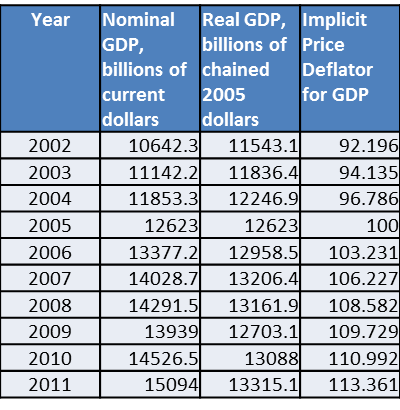
\includegraphics{images/table_2_1.png}

}

\caption{\label{fig-gdp-n-deflator}Nominal GDP, Real GDP, and Implicit
Price Deflator for GDP, U.S.A., 2002--2011}

\end{figure}%

\section{\texorpdfstring{Real Gross Domestic Product
\{\#sec-rGDP\}\index{gross domestic product!real}}{Real Gross Domestic Product \{\#sec-rGDP\}}}\label{real-gross-domestic-product-sec-rgdp}

Looking at the second column of the table in
Figure~\ref{fig-gdp-n-deflator}, we see that the nominal gross domestic
product of the United States was \$11,867.8 billion in 2004, \$12,638.4
billion in 2005, \$13,398.9 billion in 2006, \$14,077.6 billion in 2007,
and, as was mentioned earlier, \$14,441.4 billion in 2008. If one
assumes that our quality of life depends crucially on the goods and
services we produce, these ever increasing dollar figures seem like good
news.

But are they?

As nominal gross domestic product is the monetary market value of all
final goods produced, it could increase from one year to the next either
as a result of:

\begin{itemize}
\tightlist
\item
  increases in the production of various goods, or
\item
  increases in the market prices of those goods, or
\item
  increases in both production and prices.
\end{itemize}

Consequently, increases in nominal gross domestic product do not
necessarily imply increases in production. Mere inflation could make the
numbers go up and up.

Now if, by sheer luck, all prices remained unchanged during 2004--7,
then, yes, the increases in nominal GDP during that period would indeed
strongly indicate rising overall levels of production.\footnote{Even in
  this case, production might rise for some goods and fall for others.
  But it is straightforward to show that if nominal GDP rises and prices
  stay unchanged, a country would be able to buy increasing amounts of
  \emph{every} good through international trade.}

Of course, in real life, prices do not stay unchanged year after year.
But even if prices moved around a lot during 2004--7, we could still ask
a hypothetical question: What would nominal GDP have been during 2004--7
if prices had remained unchanged at 2004 levels? This is not an
unanswerable question. We know the 2004 prices of all final goods, and
we know the quantities produced, of all final goods, during the years
2004, 2005, 2006, 2007, and 2008. (Otherwise, we would not have been
able to calculate the nominal GDP figures in
Figure~\ref{fig-gdp-n-deflator}.) Therefore, we can easily calculate
what America's nominal GDP would have been in those years, had the
prices of 2004 prevailed in all years.

Indeed, data on this hypothetical measure---formally called \textbf{real
gross domestic product} or \textbf{constant-prices gross domestic
product} or \textbf{inflation-adjusted gross domestic product}---is
available for virtually every country in the world. The third column of
the table in Figure~\ref{fig-gdp-n-deflator} shows America's real gross
domestic product, calculated on the assumption that the prices of the
year 2005 prevailed in all years, for the decade 1999--2008.\footnote{Formally,
  these numbers are in ``chained 2005 dollars''. The subtleties of this
  particular method of adjusting nominal values for inflation will not
  concern us here.}

As you can see, not only did America's nominal GDP increase throughout
1999--2008, so did \emph{real} GDP. This is clear evidence of actual
increases in production. To repeat, the dollar figures in the third
column of the table in Figure~\ref{fig-gdp-n-deflator} were all
calculated on the hypothetical assumption that 2005's prices prevailed
in every year. As the same prices were used for every year's real GDP
calculations, the increases in real GDP strongly indicate overall
increases in production.

The year whose prices are being assumed hypothetically to prevail in all
years---the year 2005 in this case---is called the \textbf{base year}.
There is nothing sacrosanct about the year 2005---any other year could
have served just as well. As long as every year's GDP is calculated
using the same set of prices, we will get a measure of GDP that is not
affected by fluctuations in the overall level of prices.

In the rest of this book, all references to gross domestic product are
references to \emph{real} gross domestic product. Also, I will use the
symbol \(Y\) to denote real gross domestic product.

\subsection{Notation: Growth Rates}\label{sec-notngrowth}

Consider a variable \(x\). I will denote its \emph{current value} as
simply \(x\) and its \emph{past value} as \(x_{-1}\). Then, the
\emph{growth rate} of \(x\), which I will denote \(x_g\), can be defined
as follows: \begin{equation}\phantomsection\label{eq-growthrate}{
x_g\equiv\frac{x-x_{-1}}{x_{-1}}.
}\end{equation}

Here, \(x-x_{-1}\) represents the increase in the value of \(x\).
Therefore, \((x-x_{-1})/x_{-1}\) is the proportionate increase in the
value of \(x\) or, simply, the growth rate of \(x\). If \(x_{-1}=50\)
and \(x=60\), the increase is \(x-x_{-1}=60-50=10\). But the rate of
growth is \(x_g\equiv(x-x_{-1})/x_{-1}=(60-50)/50=0.20\).

If you want the growth rate \emph{as a percentage}, simply multiply
\(x_g\) by 100 to get \(0.20\times100=20\) percent.

To take a more concrete example, consider real gross domestic product
(\(Y\)) and its growth rate (\(Y_g\)). Figure~\ref{fig-gdp-n-deflator}
tells us that real GDP of the U.S. (in billions of chained 2005
dollars), was \$13,254.1 in 2007 and \$13,312.2 in 2008. Therefore, the
growth rate of America's real GDP in 2008 was \[
Y_g=\frac{Y_{2008}-Y_{2007}}{Y_{2007}}=\frac{13,312.2-13,254.1}{13,254.1}=0.004,
\] or \(0.004\times 100 =0.4\) percent. The real GDP growth rates for
the years 1999--2008 are given in Figure~\ref{fig-growth-inflation}.
(Can you use the data in the second and third columns of that table to
figure out the real GDP for 1998?)

\begin{figure}

\centering{

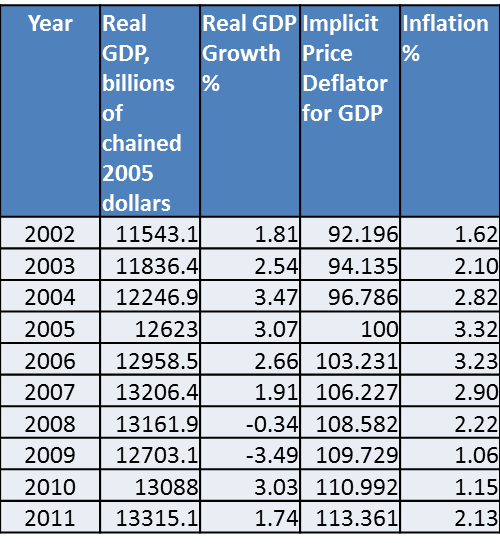
\includegraphics{images/table_2_2.png}

}

\caption{\label{fig-growth-inflation}Real GDP, GDP Growth, Implicit
Price Deflator for GDP, and Inflation, U.S.A., 2002--2011. Source:
Bureau of Economic Analysis, U.S. Department of Commerce, National
Income and Product Accounts, Tables 1.1.1, 1.1.6, and 1.1.9. Real GDP is
discussed in \textbf{?@sec-rGDP}, the growth rate of real GDP in
Section~\ref{sec-notngrowth}, the implicit price deflator in
Section~\ref{sec-IPDGDP}, and inflation in Section~\ref{sec-inflation}.}

\end{figure}%

\begin{figure}

\centering{

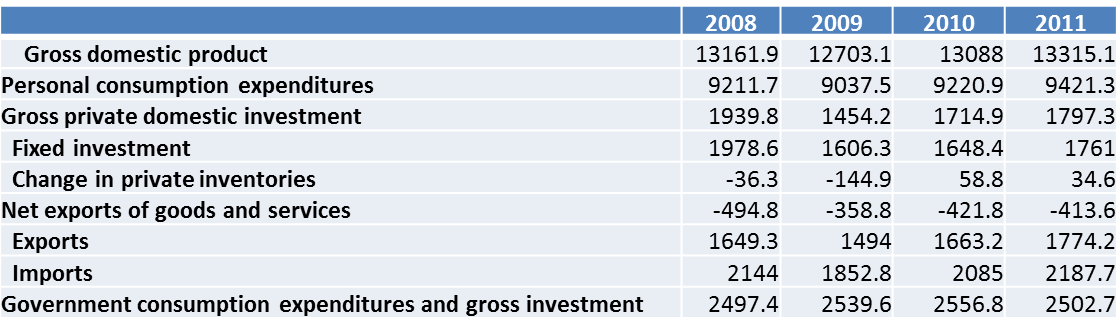
\includegraphics{images/table_2_3.png}

}

\caption{\label{fig-gdp-components}Real GDP and its Components, U.S.A.,
2008--2011, in billions of chained 2005 dollars. Source: Bureau of
Economic Analysis, U.S. Department of Commerce, National Income and
Product Accounts, Table 1.1.6.}

\end{figure}%

\begin{figure}

\centering{

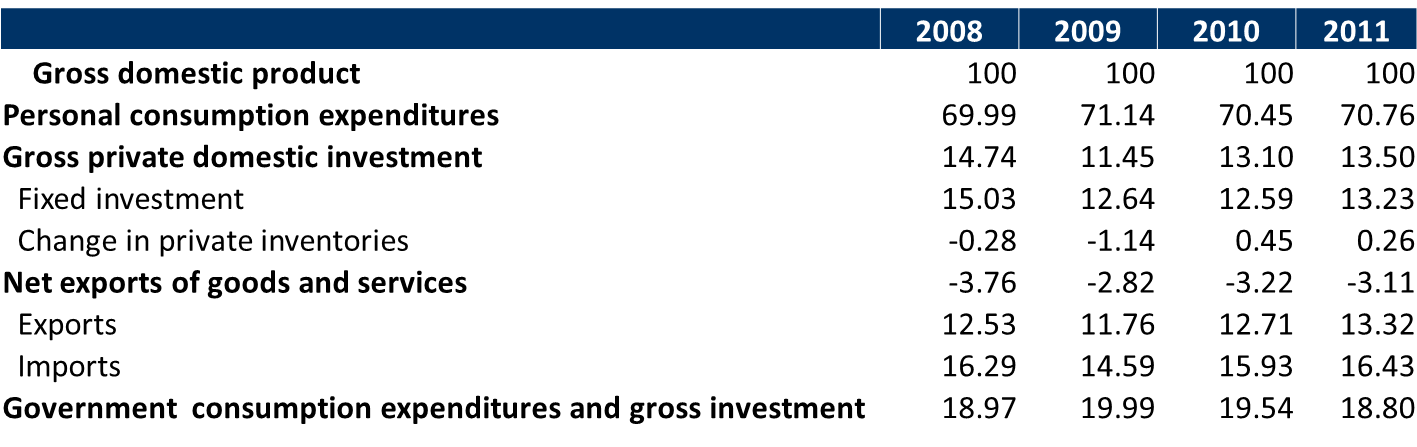
\includegraphics{images/table_2_4.png}

}

\caption{\label{fig-gdp-components-percent}Real GDP and its Components,
U.S.A., 2008--2011, as percent of Real GDP. Source: Bureau of Economic
Analysis, U.S. Department of Commerce, National Income and Product
Accounts, Table 1.1.6.}

\end{figure}%

For my discussion of the theory of international macroeconomics, I will
also use a \emph{forward-looking} definition of the growth rate of a
variable. Specifically, the \textbf{forward-looking growth rate} of
\(x\) is defined as follows:
\begin{equation}\phantomsection\label{eq-f-growthrate}{
x_g\equiv\frac{x_f-x}{x}.
}\end{equation}

Here, \(x_f\) represents the value of \(x\) in the future. Therefore,
\(x_f-x\) represents the increase in the value of \(x\). Therefore,
\((x_f-x)/x\) is the proportionate increase in the value of \(x\) or,
simply, the growth rate of \(x\).

\section{The Components of GDP}\label{sec-gdp-components}

Now that we have discussed the measurement of a country's total
production, let us look at what happens to it. Government statisticians
typically publish data not only on a country's output of final goods and
services (that is, its GDP) but also on who bought those final goods and
services. As in Figure~\ref{fig-gdp-components}, national income data
usually breaks down the big GDP number into four smaller numbers that
represent the final-goods purchases made by four major categories of
buyers:

\begin{itemize}
\tightlist
\item
  personal consumption expenditures (\(C\)),
\item
  gross private domestic investment (\(I\)),
\item
  government purchases (\(G\)), and
\item
  net exports of goods and services (\(NX\)).
\end{itemize}

In other words, Equation~\ref{eq-gdp1}, which is called the national
income identity and breaks down \emph{nominal} gross domestic product
into its components, is equally true for \emph{real} gross domestic
product: \begin{equation}
Y=C+I+G+NX.
\end{equation} \{\#eq-nii\}

\subsection{Consumption}\label{sec-consumption-nia}

\index{consumption!personal consumption expenditures}

The real (i.e., inflation-adjusted) \textbf{personal consumption
expenditures} of the residents of a country in a given year is denoted
by the symbol \(C\). In U.S. data, \(C\) consists of \emph{spending by
households} on all final goods except newly built homes. As you can see
from the U.S. data in Figure~\ref{fig-gdp-components-percent}, \(C\) is
a very large part---more than two-thirds---of GDP.

\subsection{Investment}\label{sec-investment-nia}

\index{investment!gross private domestic investment}

The real \textbf{gross private domestic investment} (or, simply,
investment) of a country is denoted by the symbol \(I\). In U.S. data,
\(I\) consists of:

\begin{itemize}
\tightlist
\item
  the purchases of fixed assets (equipment, software, and buildings) by
  businesses for use in production,
\item
  the purchases of new homes by households,\footnote{As we saw in the
    previous paragraph, this is the only category of household spending
    that is \emph{not} included in \(C\).} and
\item
  increases in inventories of unsold goods held by businesses.
\end{itemize}

Note that the inclusion of these three categories of final goods under
investment is not random. There is an underlying theme here: machines,
new buildings, stocks of as-yet-unsold goods, etc., all contribute to
our \emph{future} welfare.\footnote{The first two categories---fixed
  assets and new homes---are combined into the \emph{fixed investment}
  category in Figure~\ref{fig-gdp-components}.} The money we spend on
pizzas and backrubs, by contrast, are all about the here and now and are
included under consumption, \(C\).

As you can see from the U.S. data in
Figure~\ref{fig-gdp-components-percent}, \(I\), at less than 15\% of
GDP, is a lot less important than \(C\). And yet, because of its
tendency to fluctuate wildly, investment spending is an important cause
of the ups and downs of the overall economy.

\subsubsection{Inventories}\label{sec-inventories}

\index{investment!inventories}

The inclusion of increases in businesses' stocks of unsold goods in
\(I\) needs some justification. What's the point of including this in
\(I\)?

Keep in mind that to get an accurate picture of the health of an economy
in a given year we need to count the market value of all goods and
services produced during the year, whether or not they are sold by
December 31st of that year. Those unsold goods would not be counted in
\(C\), \(I\), \(G\), and \(NX\), if these four variables included only
the actual \emph{purchases} of final goods by households, businesses,
the government, and foreign buyers. To make sure that all goods produced
in 2008 get counted in that year's GDP---even if they are not sold in
2008---statisticians include the additions of unsold goods to
businesses' inventories (or, warehouse stocks) in \(I\).

Note that I did not say that additions to businesses' inventories of
unsold \emph{final} goods are included in \(I\); even the intermediate
goods that were produced in 2008 but not sold by the end of that year
need to be counted in that year's GDP.

Sure, as the ice cream made by Ben \& Jerry's is counted in GDP, one
should not separately count the milk that went into it because the
monetary market value of the ice cream already includes the monetary
market value of the milk. But let's complicate the story a little.
Suppose Ben \& Jerry's buys \$10 million of freshly produced milk some
time in 2008, but does not turn it into ice cream by December 31, 2008.
Instead, the milk is sitting in their freezer on that last day of 2008,
waiting to be turned into Cherry Garcia some time in 2009. This \$10
million worth of milk was produced in 2008 and, therefore, should be
included in 2008's GDP. To ensure this, the rules of GDP accounting
require that any goods that have been added to the inventories (or,
warehouse stocks of goods) of private businesses during 2008 are
\emph{final} goods and their value must be counted in the GDP for 2008.

\subsection{Government Spending}\label{sec-government-spending-nia}

\index{government spending}

Real \textbf{government expenditures} (\(G\)) is pretty much what it
sounds like; it is the inflation-adjusted monetary value of all final
goods and services bought by government entities.

Typically, governments also spend huge amounts of money on
\textbf{transfer payments} or, loosely speaking, gifts (usually to needy
people). But \(G\) includes only the money spent on the purchase of
final goods and does not include transfer payments.

\subsection{Net Exports}\label{sec-netexports-nia}

\index{net exports}

Real \textbf{exports of goods and services} (\(EX\)) is the
inflation-adjusted value of all domestically produced goods that are
bought by foreigners.\index{exports}

Real \textbf{imports of goods and services} (\(IM\)) is the
inflation-adjusted value of all foreign-made goods that are bought by
domestic residents.\index{imports}

Real \textbf{net exports} (\(NX\)) is then defined as
\(NX\equiv EX-IM\). This also goes by other names, such as \textbf{trade
surplus}, \textbf{balance on goods and services}, and, somewhat loosely,
\textbf{balance on the current account}---see
Equation~\ref{eq-balancedef}.\index{trade surplus}\index{current account!balance}
Note, therefore, that \(NX\) could be positive, zero or negative. When
\(NX\) is positive/zero/negative, the country is said to have a
\textbf{Trade Surplus/Balanced Trade/a Trade Deficit}.

\subsubsection{All exports and imports are
final!}\label{sec-exp-imp-final}

There's one more loose end in my definition of GDP that I need to tie
up. Note that in Section~\ref{sec-netexports-nia} above I defined
exports as ``all domestically produced goods that are bought by
foreigners'', not all domestically produced \emph{final} goods''.
Similarly, note that I defined imports as ``all foreign-made goods that
are bought by domestic residents'', not all foreign-made \emph{final}
goods''. Why am I including exports and imports of intermediate goods?
Suppose that American dairy farmers produce \$10 million of milk in 2008
and sell it to a Canadian ice cream company that turns the milk into ice
cream in its plant in Vancouver, also in 2008. The monetary value of the
ice cream would not be counted in America's GDP because the ice cream
was made in Canada. So, if the \$10 million of milk is regarded as an
intermediate good, it would not be counted at all in America's GDP. When
the milk is turned into ice cream by Ben \& Jerry's, the ice cream is
counted in America's GDP and, therefore, so is the milk, although
indirectly. But as for the milk that is sold to a Canadian ice cream
company, the only way to have it counted in America's GDP is to require
that \emph{anything} sold to foreigners is counted in \(EX\). Similarly,
it is straightforward to show that imports of intermediate goods should
be counted in the importing country's \(IM\).

So, here's the final corrected version---fingers crossed!---of the
definition of gross domestic product: \emph{GDP is the monetary market
value of all final goods and services produced within a country in a
given year plus the increase in its inventories of intermediate goods
plus its net exports of intermediate goods}.

\section{The National Income Identity}\label{sec-ni-identity}

To recap, we have so far defined real gross domestic product (\(Y\)),
real personal consumption expenditure (\(C\)), real gross private
domestic investment (\(I\)), real government spending (\(G\)), and real
exports (\(EX\)). It is tempting to argue that \(Y\) must be equal to
\(C+I+G+EX\). After all, \(Y\) represents all final goods that are
``Made in USA'' and any such good would have to be bought either by
American households (\(C\)), or by American businesses (\(I\)), or by
America's government (\(G\)), or by foreigners (\(EX\)). Therefore,
\(Y\) should be equal to \(C+I+G+EX\), right?

Well, not exactly. Although \(C+I+G\), which incidentally is referred to
as \textbf{gross domestic purchases}\index{gross domestic purchases},
does represent the total purchases by domestic households, businesses,
and government entities, it includes purchases of imported goods as well
as domestically produced goods. Therefore, only if we subtract the
inflation-adjusted monetary value of all imported goods (denoted by the
symbol \(IM\)) from \(C+I+G+EX\) would we get \(Y\). That is,
\(Y=C+I+G+EX-IM\).

As we saw in Section~\ref{sec-netexports-nia}, the terms \textbf{net
exports}, \textbf{trade surplus}, and \textbf{balance on goods and
services} all refer to \(NX\equiv EX-IM\), the excess of exports over
imports. Therefore, we get the \textbf{national income
identity}\index{national income identity}:
\begin{equation}\phantomsection\label{eq-ni-identity}{
Y=C+I+G+NX.
}\end{equation}

This is a reappearance of Equation~\ref{eq-gdp1} and \textbf{?@eq-nii}.

Figure~\ref{fig-gdp-components} shows data on real gross domestic
product and its components for the United States for the years 2005--8.
You can check that \(C+I+G+NX\) is indeed equal to real GDP.

A theoretically equivalent measure is \textbf{gross domestic income}.
When government statisticians measure the total value added by domestic
producers, they measure the gross domestic product (GDP). When they
measure the total income of all resources employed by domestic
producers, they measure gross domestic income (GDI). As we have seen
above, if measured with perfect accuracy, these two magnitudes should be
the same, as they are theoretically equivalent. In practice, however,
errors do creep in, and the GDP and GDI numbers tend to differ. This
difference is called the \textbf{statistical discrepancy}:
\(GDP=GDI+\hbox{statistical discrepancy}\).

\subsection{Beyond GDP: Other Measures of Total
Production}\label{sec-beyond-gdp}

Gross domestic product is not the only measure of a country's total
production, there are others.

\subsubsection{Gross National Product}\label{sec-gnp}

\index{gross national product}

Recall that a country's gross domestic product is not only the total
value added by all producers located within the country, it is also
equal to gross domestic income, which is the total income earned by the
factors of production (or, in plain language, resources) employed by all
producers located within the country.\footnote{In other words, if
  measured accurately, GDP \(=\) GDI.}

Some of the resources employed by producers located within the country
may be owned by foreign residents, and the income paid to these
resources goes, necessarily, to their foreign owners. Conversely, some
residents of the domestic country may earn income for work done for
producers located in foreign countries. A country's \textbf{net factor
income earned from foreign residents} (\(NIF\)) \emph{equals} total
income earned by domestic residents from foreign residents \emph{minus}
total income paid by domestic residents to foreign residents.

As, in some cases, it is important to know the total income earned by
the factors of production owned by a country's residents, we often pay
attention to a country's gross national product (GNP):
\begin{equation}\phantomsection\label{eq-gnp}{
\hbox{GNP}=\hbox{GDP}+\hbox{NIF}.
}\end{equation}

A theoretically equivalent measure is gross national income:
\(GNI=GDI+NIF\). Recall from Section~\ref{sec-ni-identity} that although
GDP and GDI are theoretically the same, and would be equal if accurately
measure, in practice the measured magnitudes differ slightly:
\(GDP=GDI+\hbox{statistical discrepancy}\). The same distinction needs
to be made between GNP and GNI as well; they'd be equal if measured
accurately, but in practice \(GNP=GNI+\hbox{statistical discrepancy}\).

\subsubsection{Gross National Disposable Income}\label{sec-gndi}

\index{gross national disposable income}

The residents of a country may send gifts to---and receive gifts
from---the residents of other countries. A country's \textbf{net
unilateral transfers of income from foreign residents} (NUT) is defined
as gifts received \emph{minus} gifts given. Gross national disposable
income (GNDI) is then defined as
\begin{equation}\phantomsection\label{eq-gndi}{
\hbox{GNDI}=\hbox{GNI}+\hbox{NUT}.
}\end{equation}

Recall that gross domestic product is denoted by the symbol \(Y\). In
practice, the statistical discrepancy between GDP and GDI (or between
GNP and GNI) is small. Moreover, net factor income earned from foreign
residents (NIF) and net unilateral transfers of income from foreign
residents (NUT) tend to be small too. As a result, the differences
between GDP, GDI, GNP, GNI, and GNDI are, for most practical purposes,
small enough to be ignored. Consequently, to keep the discussion simple,
I will use the symbol \(Y\) to refer to \emph{all} these different ways
of measuring a country's total value added, total income, and total
expenditure.

\subsubsection{National Income Identity, Revisited}\label{sec-nii-2}

\index{national income identity}

Recall from Equation~\ref{eq-ni-identity} that \[ Y=C+I+G+NX.\]
Therefore, \[Y+\hbox{NIF}+\hbox{NUT}=C+I+G+NX+\hbox{NIF}+\hbox{NUT}.\]
It is clear from equations Equation~\ref{eq-gnp} and
Equation~\ref{eq-gndi}, the last equation can be re-written as \[
\hbox{GNDI}=C+I+G+(NX+\hbox{NIF}+\hbox{NUT}). 
\]

As we will see in the next chapter's discussion of balance of payments
accounting, the expression within parentheses in the last equation is
called the \textbf{balance on the current account} or, simply the
current account (CA). The equation above then yields a slightly updated
version of the national income identity:
\begin{equation}\phantomsection\label{eq-nii-ca}{
\hbox{GNDI}=C+I+G+CA.
}\end{equation}

The reader should be warned, however, that I will use the terms net
exports (\(NX\)) and current account balance (\(CA=NX+NIF+NUT\))
interchangeably throughout this book, because---as was pointed out a
short while back in Section~\ref{sec-gndi}---both \(NIF\) and \(NUT\)
tend to be small in magnitude.

\section{Prices and Inflation}\label{sec-p-pi}

Inflation is a topic of major concern in economics as well as in our
daily lives. Therefore, it is important to understand what causes it and
how it can be controlled. But before we can get to that, we need to
discuss how inflation is measured.

The measurement of inflation can be quite tricky. While the prices of
some goods may rise from one year to the next, the prices of other goods
may fall. In such cases, one needs to come up with \emph{one} number
that summarizes the \emph{overall} change in prices.

\subsection{The Implicit Price Deflator for GDP}\label{sec-IPDGDP}

\index{gross domestic product!implicit price deflator for}

Suppose you recently spent a day in Boston followed by a day in San
Antonio. You ate the same meals in both cities, bought the same
newspaper, rented the same type of car, and stayed in identical hotels.
Nevertheless, you ended up spending 10\% more in Boston. Why? You did
not buy more stuff in Boston; in fact, you bought exactly the same
things in both cities. Therefore, the only explanation is that prices
were higher overall in Boston. Some things may be cheaper in Boston and
some other things may be cheaper in San Antonio. But it is reasonable to
conclude---from your own limited experience in the two cities---that the
overall level of prices was 10\% higher in Boston relative to San
Antonio.

Now consider another hypothetical example. Suppose you spent both
October 1, 2005 and October 1, 2006 in Boston and during both visits you
bought the exact same things, used the same transportation, and stayed
in identical hotel rooms. And yet, you ended up spending 4\% more in
2006 than in 2005. Using the same logic as in the last paragraph, we can
conclude that although individual items' prices may have changed at
different rates, the overall level of prices in Boston rose 4\% in 2006
relative to 2005.

In fact, you don't even have to visit Boston on two different dates.
After your October 1, 2006 visit, you could dig up data on the prices
that you would have paid if you had visited Boston a year earlier and
bought the same goods and services that you bought during your October
1, 2006 visit, and you would have again reached the conclusion that the
overall level of prices rose 4\% in Boston in 2006. And that, by and
large, is what government statisticians do to measure the rates of
change of the overall level of prices in the US and other countries.

One way to measure the overall level of prices is to compare the nominal
GDP and the real GDP for a particular year. We see in
Figure~\ref{fig-gdp-n-deflator}\} that in 1999 America's nominal GDP was
\$9,353.5 billion and America's real GDP, with base year 2005, was
\$10,779.8 billion. Stated differently, in 1999 America's nominal GDP
was 86.8\% of America's real GDP: \begin{eqnarray*} 
\frac{\hbox{Nominal GDP in 1999}}{\hbox{Real GDP in 1999 with base year 2005}}\times 100&=&\frac{9,353.5}{10,779.8}\times 100\\
&=& 86.8.
\end{eqnarray*} So, at 1999 prices, the dollar value of all final goods
produced in the U.S. in 1999 was \$9,353.5 billion, whereas, at 2005
prices, the dollar value of the exact same goods was \$10,779.8 billion.

Now, how could one dollar value of the final goods made in 1999 be
different from the other dollar value of the exact same goods? As the
quantities used in the nominal GDP calculation are the same as the
quantities used in the real GDP calculation, these two dollar values
must be different because they use different \emph{prices}.

More precisely, the only possible reason why America's nominal GDP in
1999 is 86.8\% of America's real GDP in 1999 must be that the prices
that prevailed in 1999, which are the ones that were used in the
calculation of nominal GDP, were, in an overall sense, 86.8\% as high as
the prices that had prevailed in 2005, which are the ones that were used
in the calculation of real GDP.

It would be incorrect to conclude that \emph{all} final goods were
86.8\% as pricey in 1999 as in 2005. For apples, the 1999 price may have
been 80\% of the 2005 price. For haircuts, the 1999 price may have been
130\% of the 2005 price. For gas at the pump, the 1999 price may have
been 99\% of the 2005 price. But it is reasonable to say that in an
overall sense the 1999 prices were 86.8\% as high as the 2005 prices
because the final goods that were produced in America in 1999 were only
86.8\% as valuable at 1999 prices than at 2005 prices.

Thus, by comparing the nominal and real GDP values for a particular year
we are able to measure how that year's prices as a whole measure up
relative to the base year's prices. Formally, the

\begin{equation}\phantomsection\label{eq-IPDGDP}{
\hbox{Implicit Price Deflator for GDP in year $n$ with base year $m$} = \frac{\hbox{Nominal GDP in year $n$}}{\hbox{Real GDP in year $n$ with base year $m$}}\times 100
}\end{equation} shows what the overall level of final goods' prices in
year \(n\) was as a percentage of the base year's overall price level.
More compactly, \begin{equation}\phantomsection\label{eq-IPDGDP}{ 
\hbox{Implicit Price Deflator}=
\frac{\hbox{Nominal GDP}}{\hbox{Real GDP}}\times 100.
}\end{equation}

The fourth column in Figure~\ref{fig-gdp-n-deflator}\} shows America's
implicit price deflator for GDP (IPDGDP) for the 1999--2008 decade.
Specifically, it shows that the overall level of prices in 1999 was
86.8\% of the overall level of prices in 2005. Similarly, the overall
level of prices in 2005 was 100\% of the overall level of prices in
2005---what a shocker!---and the overall price level in 2007 was 106.2\%
of the overall level of prices in 2005.\footnote{If you saw
  Figure~\ref{fig-gdp-n-deflator}, but without any information about
  2005 being the base year in the heading of the third column, would you
  still be able to figure out that 2005 is the base year?}

In the remainder of these lectures, I will represent the overall price
level for a particular year not by the implicit price deflator for GDP
but by a very slightly different version of it: \begin{eqnarray}
P&=&\frac{\hbox{Implicit Price Deflator for GDP}}{100}\nonumber \\
&=&\frac{\hbox{Nominal GDP}}{\hbox{Real GDP}}\times\frac{100}{100}\nonumber \\
&=&\frac{\hbox{Nominal GDP}}{Y}.
\end{eqnarray} \{\#eq-P\} Note that \textbf{?@eq-P} comes from equation
Equation~\ref{eq-IPDGDP}.

In other words, while real GDP is represented by the symbol \(Y\), the
overall level of prices is denoted by the symbol \(P\), and nominal GDP
is given by \begin{equation}\phantomsection\label{eq-nomGDP}{
\hbox{Nominal GDP}=P\times Y.
}\end{equation}

\subsection{The Consumer Price Index}\label{sec-cpi}

\index{consumer price index}

The implicit price deflator for GDP is not the only one-number
representation of the overall level of the prices of the innumerable
goods that are bought and sold in a modern economy. Indeed, it may not
even be the most popular method: a frequently cited alternative measure
of the overall level of prices is the \textbf{consumer price index}.

Whereas the implicit price deflator for GDP is (100 times) the value of
the current year's output of final goods at the current year's prices
divided by the value of the same set of goods at the base year's prices,
the consumer price index is (100 times) the value of \emph{a fixed
bundle of goods that represents the purchases of a }typical consumer* at
the current year's prices divided by the value of that same bundle of
goods at the base year's prices.

Although \textbf{?@eq-P} sees the overall price level, \(P\), as the
implicit deflator for GDP divided by 100, you may, if you wish, think of
\(P\) as the consumer price index divided by 100. In practical terms,
these two measures of the overall price level tend to move in sync most
of the time.\footnote{However, an increase in the price of M16 rifles,
  which are usually bought by a country's armed forces but not by its
  typical consumer---not yet anyway!---would raise the value of the GDP
  deflator but not the CPI.}

\subsection{Inflation}\label{sec-inflation}

\index{inflation!measurement}

Finally, how do we measure inflation? Inflation is defined simply as the
growth rate of the overall level of prices, where the term `growth rate'
is as it is defined in Section~\ref{sec-notngrowth}. I will denote
inflation by the symbol \(\pi\), which is the lower-case Greek letter
`pi'. Denoting the past value of the overall price level by the symbol
\(P_{-1}\), we can use equation Equation~\ref{eq-growthrate} to express
inflation as follows:
\begin{equation}\phantomsection\label{eq-inflation}{
\pi\equiv\frac{P-P_{-1}}{P_{-1}}\equiv\frac{P}{P_{-1}}-1.
}\end{equation} The increase in the overall price level is \(P-P_{-1}\).
But the proportionate increase in \(P\) is \((P-P_{-1})/P_{-1}\). And to
express inflation as a \emph{percentage}, one has to multiply \(\pi\) by
100.

For example, the annual inflation rate for, say, 2004 is
\begin{eqnarray} 
\lefteqn{\hbox{Inflation during 2004}}\nonumber \\
&=&\frac{P_{2004}-P_{2003}}{P_{2003}}\times 100\\
&=&\frac{\hbox{IPDGDP}_{2004}-\hbox{IPDGDP}_{2003}}{\hbox{IPDGDP}_{2003}}\times 100\\
&=&\frac{96.77-94.1}{94.1}\times 100\nonumber \\
&=&2.8 \hbox{ percent}.\nonumber 
\end{eqnarray}\{\#eq-inflation2004\}

America's annual inflation rates, as defined above, are shown in
Figure~\ref{fig-growth-inflation} for 1999--2008. Although these
inflation numbers are calculated based on the implicit price deflator
for GDP as the price level, one could also think of inflation as the
annual percentage increase in the consumer price index, which has been
discussed above in Section~\ref{sec-cpi}. In practical terms, this does
not make much difference to inflation data, especially over longer
periods, as you can see in Figure~\ref{fig-inflation}. Over short
periods of time, however, inflation measures based on the consumer price
index are more volatile, as can be seen in
Figure~\ref{fig-cpi-volatile}\}.

\begin{figure}

\centering{

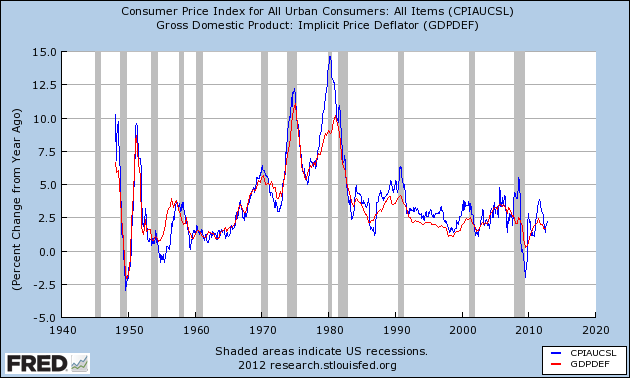
\includegraphics{images/cpiaucsl-gdpdef-fredgraph.png}

}

\caption{\label{fig-inflation}Inflation: Two Measures The red graph
represents US inflation measured by the year-on-year percentage change
in the implicit price deflator for GDP. The blue graph uses the consumer
price index (for all urban consumers) instead. Source: Data on the
implicit price deflator for GDP was downloaded from
\url{http://research.stlouisfed.org/fred2/series/GDPDEF} and data on the
consumer price index was downloaded from
\url{http://research.stlouisfed.org/fred2/series/CPIAUCSL}, both on
November 25, 2012.}

\end{figure}%

\begin{figure}

\centering{

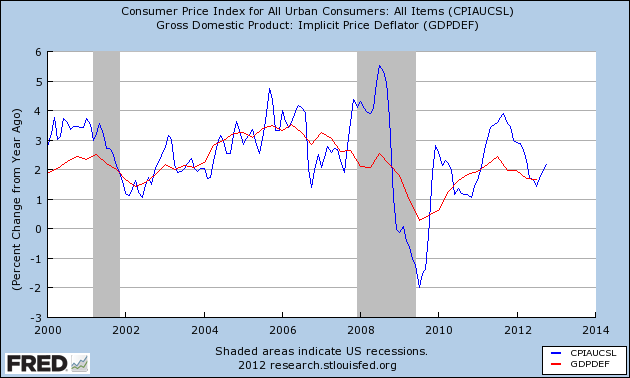
\includegraphics{images/cpiaucsl-gdpdef-fredgraph-b.png}

}

\caption{\label{fig-cpi-volatile}\textbf{Inflation: CPI Is More
Volatile} The red graph represents US inflation measured by the
year-on-year percentage change in the implicit price deflator for GDP.
The blue graph uses the consumer price index (for all urban consumers)
instead. This chart focuses on the 21st century and highlights the
volatility of the CPI. Source: Data on the implicit price deflator for
GDP was downloaded from
\url{http://research.stlouisfed.org/fred2/series/GDPDEF} and data on the
consumer price index was downloaded from
\url{http://research.stlouisfed.org/fred2/series/CPIAUCSL}, both on
November 25, 2012.}

\end{figure}%

\bookmarksetup{startatroot}

\chapter{Balance of Payments Accounts}\label{sec-bopacc}

A country's balance of payments\index{balance of payments} account for,
say, 2003 summarizes all economic transactions that took place between
its residents and foreign residents during 2003.

The balance of payments accounts consist of the \textbf{current
account}, the \textbf{capital account}, and the \textbf{financial
account}.

\section{The Current Account}\label{sec-curacc}

To keep things simple, let's assume that in every transaction there is
one person who hands over some goods, services or assets and another
person who pays (for those goods, services or assets) with
cash.\footnote{By assets I mean \emph{non-cash} assets. It is possible
  that a US resident might buy some Swedish kroner, which is a cash
  asset, and just hang on to it. But I will keep things simple by
  assuming that a US resident who buys some Swedish kroner would
  immediately spend it on some goods, services or non-cash assets (such
  as stocks, bonds, the title to a house, etc.) perhaps because she has
  no use for Swedish kroner in the US. As a result, it makes sense to
  assume that when cash is offered as payment, it is to buy some
  non-cash asset. Moreover, although it is possible for Alan to hand
  over some IBM shares to Betty and get some Google shares in return,
  not much realism is lost by assuming that Alan gets cash for his IBM
  shares and then uses the cash to buy Google shares from Betty.}

Transactions in which \emph{goods or services} are traded between
\emph{residents} of America and \emph{residents} of other countries are
summarized in America's current
account\index{balance of payments!current account}.

\section{The Capital Account}\label{sec-capacc}

The balance of payments accounts also includes the capital
account\index{balance of payments!capital account}. But I will ignore it
because it usually involves small sums of money and is not important for
my purposes. According to \emph{International Economics}, 2nd edition,
by James Gerber (Addison Wesley; Boston, MA; 2002; page 176), ``The
capital account includes transfers of specific types of capital, such as
debt forgiveness, the personal assets that migrants take with them when
they cross international boundaries, and the transfer of real estate and
other fixed assets, such as the transfer of ownership of a military base
or an embassy.''

Prior to 1996 what we now call the financial account used to be called
the capital account and used to include what we now call the capital
account.

To repeat, I will ignore the capital account. That is, unless I make an
explicit statement to the contrary, I will assume that none of the types
of international transactions that are formally classified under the
capital account are actually taking place.

\section{The Financial Account}\label{sec-finacc}

Transactions in which \emph{assets} are traded between residents of
America and residents of other countries are summarized in America's
financial account\index{balance of payments!financial account}.

An \textbf{asset}\index{asset} is pretty much anything that you can buy
today (if you have some surplus cash) and sell later (if you need some
extra cash). If your asset provides some service to someone while you
are its owner, you can earn an \emph{income} from your asset. For
example, if an American buys a house in Germany, she would be buying an
\emph{asset}. And the rental income she earns by renting out the house
is her \emph{asset income}. If an American buys a German company's
stock, she would be buying an \emph{asset}. And the dividend income she
earns (as long as she owns the stock) is her \emph{asset income}. If an
American puts money in a German bank, that bank account is an
\emph{asset} that will periodically yield interest \emph{income}.

Interestingly, while \emph{international asset trades are recorded in
the financial account} of a nation's balance of payments, the
\emph{income earned from those assets are considered to be payments for
services rendered by the assets and are, therefore, recorded in the
current account}. So, an American's purchase of a house in Germany will
be recorded in the financial account and any subsequent rental income
from that house will be recorded in the current account.

The financial account includes the \textbf{Official Reserve Transactions
Account}\index{balance of payments!financial account!Official Reserve Transactions Account}.
Most countries have \textbf{central banks}\index{central banks} that
design and carry out their monetary policies. For example, America's
central bank is the Federal Reserve (or, simply, the
Fed\index{central banks!Fed, the}). Central banks often buy and/or sell
assets. For example, the Bank of
Japan\index{central banks!Japan, Bank of} (i.e., Japan's central bank)
may buy U.S. Treasury bonds. It may then sell those bonds at a later
date if it needs dollars. The assets that central banks typically buy
and sell are called \textbf{reserve assets}\index{reserve assets}.
\emph{International trade in reserve assets conducted by central banks
is recorded in the official reserve transactions account}.

\section{Credits, Debits, and
Balances}\label{sec-credits-debits-balances}

Recall that all economic transactions that take place between a
country's residents and the residents of other countries are recorded in
the country's current, capital, and financial accounts. The recording of
these transactions follows strict rules. This section presents a
simplified look at the rules of balance of payments accounting.

\subsection{Which Transactions Are Recorded as
Credits?}\label{sec-credits}

Recall from Section~\ref{sec-curacc} that I have assumed that in every
transaction there is one person who hands over goods, services or
non-cash assets (such as stocks and bonds) and another person who pays
with cash or check (i.e., money; to economists, both currency and checks
count as money). Any transaction resulting in a receipt of money from
foreigners is entered in the balance of payments accounts as a
credit\index{balance of payments!credits} and is given a positive
(\(+\)) sign. In other words, any transaction in which we sell (i.e.,
\emph{export}) goods, services or assets to foreigners is recorded as a
\emph{credit}.

\subsection{Which Transactions Are Recorded as
Debits?}\label{sec-debits}

Any transaction in which we pay money to foreigners is entered in the
balance of payments accounts as a
debit\index{balance of payments!debits} and is given a negative (\(-\))
sign. In other words, \emph{imports} of goods, services and assets are
recorded as \emph{debits}.

\section{Accounting Rules: Examples}\label{sec-accex}

Here are some examples that illustrate the rules of balance of payments
accounting that I have discussed above:

\begin{itemize}
\tightlist
\item
  The sale (i.e., export) of a U.S. car to Germany is a \emph{credit} in
  the U.S. \emph{current} account.
\item
  An American's purchase (i.e., import) of a house in Germany is a
  \emph{debit} in America's \emph{capital} account.
\item
  The rental income earned by an American from her house in Germany is
  seen as the \emph{export} of housing services from America to Germany
  and is, therefore, a \emph{credit} in America's \emph{current}
  account.
\item
  When a German deposits some extra cash in his New York bank account,
  it is seen as the purchase by the German (and, therefore, an
  \emph{export} by America) of an American asset (in this case, the
  increased value of the bank account) and is recorded as a
  \emph{credit} in America's \emph{financial} account.
\end{itemize}

Note again that \emph{credits are always exports} of goods, services or
assets and \emph{debits are always imports}.

\subsection{\texorpdfstring{What Is the \emph{Balance} on an
Account?}{What Is the Balance on an Account?}}\label{sec-balance}

\emph{The total of all credits minus the total of all debits in an
account or sub-account is called its
balance}\index{balance of payments!balance}. The balance could be
positive, zero, or negative.

Since credits are exports and debits are imports,
\begin{equation}\phantomsection\label{eq-balancedef}{
\mbox{Balance} = \mbox{Credits} - \mbox{Debits} = \mbox{Exports} - \mbox{Imports} = \mbox{Net Exports}.
}\end{equation} In particular, \emph{our current account balance is our
net export of goods and services} and \emph{our financial account
balance is our net export of assets}.

Most internationally traded assets are paper assets such as stocks and
bonds. Unlike the purchase of, say, a house, the purchase of a stock or
a bond does not involve the exchange of some tangible commodity. The
purchase of stocks and bonds simply entitle the buyer to future income.
If you buy Microsoft stock, Microsoft will get your money \emph{today}
and you will receive a share of Microsoft's \emph{future} profits (as
long as you keep the stock). If you buy a bond from AT\&T, AT\&T will
get your money \emph{today} and you will get regular \emph{future}
payments of some amount specified on the bond. Notice that in both of
these last two cases, what you are really doing is \emph{lending} some
of your money to others \emph{today} in the expectation that they will
pay you in the \emph{future}. When you buy Microsoft stock, you are
lending money to Microsoft. When you buy AT\&T bonds, you are lending
money to AT\&T. Similarly, the sale of stocks (by, say, Microsoft) and
bonds (by, say, AT\&T) is simply a way for these companies to borrow
money.

Applying this idea to international asset trades, \emph{America's sale
(or, export) of stocks and bonds to foreigners during 1999 is equal to
the amount America borrowed from foreigners during 1999 and America's
purchase (or, import) of stocks and bonds from foreigners during 1999 is
equal to the amount America loaned to foreigners during 1999. Therefore,
our financial account balance for 1999 is equal to the increase in our
net indebtedness to foreigners during 1999}.

\[
\lefteqn{\mbox{Financial Account Balance in 1999}}\\
&=&\mbox{Financial Account Credits}-\mbox{Financial Account Debits}\nonumber\\
&=&\mbox{Assets Exports}-\mbox{Assets Imports}\nonumber\\
&=&\mbox{Borrowing from foreigners in 1999}-\mbox{Lending to foreigners in 1999}\nonumber\\
&=&\mbox{Increase in our net indebtedness in 1999.}\nonumber
\] \{eq-intdebt\}

If, for example, our financial account balance during 1999 was +\$100
billion, then we borrowed \$100 billion more from foreigners than we
lent them, and, so, our indebtedness to foreigners increased in 1999 by
\$100 billion.

And, by the way, that increase of \$100 billion in our foreign debt
could have happened in several different ways: For example, the amount
we owe them could have gone up from \$500 billion to \$600 billion or
the amount they owe us could have gone down from \$300 billion to \$200
billion or their debt to us of \$25 billion may have turned into our
debt to them of \$75 billion during 1999.

If, on the other hand, our financial account balance was -\$150 billion,
then our net indebtedness to foreigners decreased by \$150 billion.
\emph{Therefore, a positive financial account balance means an increase
in our international indebtedness and a negative financial account
balance means a decrease in our international indebtedness}.

\section{Balance of Payments Identity}\label{sec-curcap}

Now that we have seen how the balances in the current, capital, and
financial accounts are defined, it is necessary to see how the three
balances are related. It turns out that \emph{the balances of the
current, capital, and financial accounts must always sum to zero}:

\begin{equation}\phantomsection\label{eq-balancedpayments}{
\mbox{current account balance} + \mbox{capital account balance} + \mbox{financial account balance} \equiv 0.
}\end{equation}

So, if we ignore the typically tiny capital account, if the current
account balance is \(-\)\$5000, then the financial account balance would
have to be +\$5000, and vice versa.

To see the logic behind Equation~\ref{eq-balancedpayments}, let the
current account balance be \(-\)\$5000. In other words, our net export
of goods and services is \(-\)\$5000. That is, we bought \$5000 more
goods and services from foreigners than we sold to them. This raises a
question: How could it have happened? Are we living on the charity of
foreigners? Why would they give us \$5000 more stuff than we gave them?
The answer is that the foreigners will let us have an additional \$5000
worth of \emph{goods and services} as long as we give them an additional
\$5000 of \emph{assets}. That is, our net export of goods and services
may be \(-\)\$5000 as long as our net export of assets is \(+\)\$5000.
Therefore, recalling from Equation~\ref{eq-balancedef} that ``net
export'' is also called ``balance'', our current account balance can be
\(-\)\$5000 as long as our financial account balance is \(+\)\$5000.

We saw in Section~\ref{sec-balance} that a positive financial account
balance reflects an increase in our net indebtedness to foreigners.
Therefore, Equation~\ref{eq-balancedpayments} means that we can import
more goods and services than we export, as long as we understand that
there will be an increase in our net indebtedness.

Another way to see this is to recognize that every international
transaction will necessarily involve a credit in one of the two
accounts---i.e., in either the current account or the financial
account---and a debit of equal size in the other account.

Consider an example. Suppose a German buys an American car for \$50,000.
This is a credit in the current account and, therefore, our current
account balance increases by \$50,000. Now, where would the German buyer
get those dollars? There are several possibilities:

\begin{itemize}
\tightlist
\item
  He has a bank account in New York from which he pays the \$50,000. In
  this case, following example 4 in Section~\ref{sec-accex} above, we
  can see that this is a debit of \$50,000 in our financial account. So,
  our financial account balance decreases by \$50,000.
\item
  He sells some of his U.S. assets (such as real estate or stocks or
  bonds) and uses that money to buy his car. Again, a glance at examples
  2 and 4 in Section~\ref{sec-accex} will show you that this has the
  same effect as in the previous case: our financial account balance
  decreases by \$50,000.
\item
  He buys \$50,000 from an American who needed Euros to open a bank
  account in Germany. As you can tell from example 4 in
  Section~\ref{sec-accex}, this is a \$50,000 debit in our financial
  account. So, again, our financial account balance decreases by
  \$50,000.
\end{itemize}

The point of these examples is that if a transaction causes our current
account balance to \emph{increase} by \$50,000, then it must
simultaneously involve another transaction that causes our financial
account balance to \emph{decrease} by the same amount, irrespective of
the gory details of the transaction.

Similarly, it can be shown that any transaction that \emph{decreases}
our current account balance by \$40,000 will simultaneously be
accompanied by other transactions that will \emph{increase} our
financial account balance by \$40,000.

More generally, any transaction that changes the balance on any of these
two accounts will be accompanied by other transactions that change the
balance on the other account by the same amount but in the opposite
direction. Hence, the current account balance plus the financial account
balance must always be zero.

In other words---using the idea that the balance on an account is equal
to the net exports on that account; see equation
Equation~\ref{eq-balancedef} --- the net exports of goods and services
must equal the net imports of assets, and vice versa.

\bookmarksetup{startatroot}

\chapter{Exchange Rates}\label{sec-exrates}

The currency of a country is valuable, even to residents of other
countries. Non-Americans may wish to buy dollars (with their own
respective currencies), in order to buy American goods, services or
assets.\footnote{By ``non-Americans'' I mean residents of countries
  other than the United States. Similarly, by ``Americans'' I mean
  residents of the United States, citizens or not.} Similarly, Americans
may be willing to pay dollars to buy foreign currencies. The
institutions that enable people to trade one currency for another are
called \textbf{foreign exchange
markets}\index{markets!foreign exchange}. The amount of currency \(A\)
(say, the US dollar) that will have to be paid as the price of one unit
of currency \(B\) (say, the euro) in the foreign exchange market is the
\textbf{exchange rate}\index{exchange rate} of currency \(B\) in terms
of currency \(A\).

\section{Nominal Exchange Rates}\label{sec-nomexrates}

The answer to the question ``What are \emph{nominal} exchange rates?''
is actually the same as the answer to the question ``What are exchange
rates?''. The nominal exchange
rate\index{exchange rate!nominal exchange rate} of the euro in terms of,
say, the US dollar is the price of a euro in dollars. The word
``nominal'' is sometimes added simply to serve as a reminder that there
exists another kind of exchange rate: the real exchange rate.

In this lecture, I will typically consider two currencies: the
\emph{domestic} currency and the \emph{foreign} currency. I will use the
symbol \(E\) to denote \textbf{the price of the foreign currency
measured in units of the domestic currency}. So, if the domestic
currency is the US dollar and the foreign currency is the British pound,
and if one pound is worth \$2.00, then \(E = 2.00\). If one US dollar is
worth 100 Japanese yen, then \(E=0.01\). (Why?)

\section{Real Exchange Rates}\label{sec-realexrates}

The real exchange rate\index{exchange rate!real exchange rate} is
\emph{the (average) price of foreign-made goods and services measured in
units of domestically produced goods and services}. It is denoted by the
symbol, \(q\), of the lower case Greek letter ``epsilon'', and it is
computed by the following equation:
\begin{equation}\phantomsection\label{eq-q}{
q=\frac{E\cdot P^*}{P}
}\end{equation}

Here, \(P\) (respectively, \(P^*\)) represents \textbf{the average level
of prices} of goods and services made in the domestic (respectively,
foreign) economy. By ``average level of prices'' I mean some sort of
price index such as the implicit price deflator for GDP or the consumer
price index\index{consumer price index}.\footnote{These variables were
  discussed in Section~\ref{sec-p-pi}. See in particular
  \textbf{?@eq-P}.}

To see why Equation~\ref{eq-q} does measure the relative price of
foreign goods in units of domestic goods, consider a world in which
wheat is the only traded good. Consider ``Made in USA'' wheat and ``Made
in France'' wheat. Let the price of ``Made in USA'' wheat be \$2.00 per
pound; that is, let \(P=2\). Let the price of ``Made in France'' wheat
be \EUR{6.00} per pound; that is, let \(P^*=6\). Let the price of one
euro be \$2.00; that is, let \(E=2.00\). Note that the price of ``Made
in France'' wheat is \EUR{6.00} which is worth \$12.00. Note also that
\$12.00 would buy you six pounds of ``Made in USA'' wheat. Therefore,
one pound of ``Made in France'' wheat has the same market value as six
pounds of ``Made in USA'' wheat. That is, the real exchange rate of
``Made in France'' wheat is six pounds of ``Made in USA'' wheat. In
symbols, \(q=6\).

Let us now see if the formula in Equation~\ref{eq-q} gives the same
answer. If we substitute \(P=2\), \(P^*=6\) and \(E=2.00\) in
Equation~\ref{eq-q}, we get \(q=(2.00\times 6)/2 =6\), which is exactly
the real exchange rate we got in the last paragraph.

Note that the real exchange rate, being the price of foreign-made goods
(measured in units of domestically produced goods), is a measure of the
foreign economy's
competitiveness\index{exchange rate!real exchange rate!competitiveness}.
The higher the value of \(q\), the less attractive foreign-made goods
would be (to domestic buyers) and the more attractive domestically
produced goods would be (to foreign buyers).

\subsection{Notation: Foreign Country Variables}\label{sec-notnfornvar}

As I did in the case of \(P^*\) in Section~\ref{sec-realexrates}, I will
use an asterisk (*) as a superscript to mark all foreign variables;
i.e., all variables describing the rest of the world.

\section{What Are Spot Exchange Rates?}\label{sec-spotexrates}

The spot exchange rate is just another way of refering to the exchange
rate that I discussed earlier in Chapter~\ref{sec-exrates}. Today's spot
exchange rate\index{exchange rate!spot exchange rate} of, say, the
Japanese yen in terms of the US dollar is the price---of a yen, in
dollars---at which any dollar-yen exchange would take place today. This
is, therefore, just another, fancier name for the \(E\) that was defined
earlier. The word ``spot'' is sometimes added simply to serve as a
reminder that there exists another kind of exchange rate: the Forward
Exchange Rate.

\section{What Are Forward Exchange Rates?}\label{sec-forwardexrates}

Today's ``30-day forward exchange
rate''\index{exchange rate!forward exchange rate} of the yen in terms of
the US dollar is the price---of a yen, in dollars---that you would have
to pay for any dollar-yen exchange you agree \emph{today} to do \emph{30
days later}. Only the agreement is signed today; the actual exchange of
currencies takes place 30 days later. Let us denote the 30-day forward
exchange rate of the foreign currency in terms of the domestic currency
by \(f_{30}\). So, if \(f_{30} = 0.095\) US dollars today, you can sign
an agreement today to sell \$9.50 thirty days later in exchange for 100
yen.

But why would anyone do such a thing? That is, why would one sign an
agreement \emph{today} to make a currency exchange \emph{thirty days
later?} Well, by trading currencies on the forward exchange market, one
can \emph{avoid exchange rate uncertainty}. Suppose you will have to pay
someone 100 yen thirty days from today. If you sign a forward-market
agreement today and if \(f_{30}=0.095\), you'll know that you'll need
exactly \$9.50 thirty days later to make your 100 yen payment. You could
instead wait 30 days, go to the foreign exchange spot market and buy 100
yen at whatever spot-market exchange rate prevails at that date. But
that would be a gamble: you could end up paying \$9.50 or more than
\$9.50 or less than \$9.50 depending on what the spot rate is at that
date.

\subsection{Forward Exchange Rates and
Expectations}\label{sec-forward-exp}

It can be shown that the 30-day forward exchange rate of the yen is a
proxy measure of what people currently expect the spot-market value of
the yen will be 30 days in the future. That is, if \(f_{30} = 0.095\) US
dollars per yen today, then it is a safe bet that people today expect
that one yen will be worth \$0.095 thirty days later in the spot market.
Why?

Recall that the nominal exchange rate (\(E\)) is the current spot-market
value of one unit of the foreign currency. Using the notational rule set
out in Section~\ref{sec-notngrowth}, let \(E_f\) denote the
\emph{future} spot-market value of one unit of the foreign currency.
And, finally, let \(E_f^e\) denote the \textbf{current expectation of
the future value of the nominal exchange rate}. My claim is that
\(f_{30}\) is a good estimate of \(E_f^e\) when the future is 30 days
ahead.

To see why this is, suppose, to the contrary, that \(f_{30} = 0.095\) US
dollars per yen today, but that people today think that thirty days
later one yen will be worth \(E_f^e =0.080\) US dollars in the spot
market. Now, if people are more or less convinced that thirty days later
they would be able to buy one yen in the spot market for \$0.080, why
would they rush to the forward market today and pay \$0.095 for every
yen that they must pledge to buy thirty days later? It doesn't make
sense. If instead we had \(f_{30} = 0.095\) and \(E_f^e =0.099\), then
people would indeed want to buy yen in the forward market.

But now nobody would want to \emph{sell} yen in the forward market. To
see why, suppose you are an American exporter and you are expecting a
Japanese client to pay you in yen thirty days in the future. You could
wait till you receive the yen payment and then sell your yen on the spot
market to get dollars, or you could sell the expected receipt of yen on
the forward market \emph{today}. Which would you rather do? As the
forward value of a yen is \(f_{30} = 0.095\) and you expect that the
spot-market value will be \(E_f^e =0.099\), you will surely choose to
avoid the forward market.

To summarize, I have established that if \(f_{30} > E_f^e\) then nobody
would want to buy the foreign currency in the forward market. I have
also established that if \(f_{30} < E_f^e\) then nobody would want to
sell the foreign currency in the forward market. Therefore, the only
reasonable outcome is \(f_{30} = E_f^e\). That is, today's
forward-market price of a currency is a good estimate of what people
today expect that currency's spot-market value will be in the future.

Typically, you can't tell what people expect the future to be. But in
the case of foreign exchange rates at least, there is a way to do so!

\bookmarksetup{startatroot}

\chapter{Data}\label{data}

\section{Description}\label{description}

\section{Missing value analysis}\label{missing-value-analysis}

\bookmarksetup{startatroot}

\chapter{Results}\label{results}

\bookmarksetup{startatroot}

\chapter{Interactive graph}\label{interactive-graph}

\phantomsection\label{plot}

\bookmarksetup{startatroot}

\chapter{Conclusion}\label{conclusion}


\backmatter

\printindex

\end{document}
